\chapter{Setting the Scene for Imperfect Information}
\epigraph{
  Intelligence is a~game of~imperfect information.
  We can guess our opponent's moves, but we can't be sure until the game is over.
}{Khalid Muhammad}
\todo Uvod

\section{Extensive Form for Imperfect-Information}
\label{sec:extensive-form-imperf-info}
\epigraph{
  Education is only a~ladder to~gather fruit from the tree of~knowledge, not the fruit itself.
}{Albert Einstein}
Recall extensive forms (for perfect-information games) from Section~\ref{sec:extensive-form-perf-info}.
An~\emph{extensive form} (for an~imperfect-information game) is the usual extensive form with additional:
\begin{itemize}
  \item \textbf{c}hance player $c$ (e.~g. a~dice, the card dealer, the nature etc.).
    The set of~players is thus $P \cup \braces{c}$ and the probability corresponding to a~strategy profile~$\sigma$ includes the chance:
    \[\pi ^\sigma(h) = \prod _{i \in P \cup {c}} \pi _i ^\sigma (h)\]

  \item function $f_c$ determining the probability distribution over actions~$A(h)$ for every chance node~$h$ (i.e. $p(h) = c$).

  \item partition $\I_i$ of nodes $\braces{h \in H: p(h) = i}$, which is called the \emph{information partition} of player~$i$.
    Its element $I \in \I_i$ is an~\emph{information set} of player~$i$ and $I(h) \in \I_i$ (with $p(h) = i$) denotes the information set containing $h$.

    An information set represents grouping of histories that are indistinguishable from $i$'s point of view.
    In the game of poker, for example, this might be because of  opponents' hidden cards.
\end{itemize}
\noindent
\begin{figure}[H]
  \centering
  \scriptsize
  \def\svgwidth{.7\textwidth}
  \input{../img/strategic-form-tree.pdf_tex}
  \def\captionTitle{An~imperfect-information game tree with information sets}
  \caption[\captionTitle]{\captionTitle{} \\(\cite[p.~67]{AGT07})}
  \label{fig:strategic-form-tree}
\end{figure}
\noindent
There are further notions related to extensive-form games:
\begin{itemize}
  \item A~(behavior) \emph{strategy}~$\sigma_i$ of player~$i$ gives a~probability distribution over $A(I)$ at every $I \in \I_i$, and $\pi ^\sigma (I, a)$ is the probability of action $a$ at the information set~$I$.
    Again, $\Sigma_i$ denotes the set of all possible strategies for player~$i$.

  \item $\sigma | _{I \goto a}$ denotes the strategy identical to $\sigma$ with the only one exception:
    the action~$a$ is always played at the information set~$I$.

  \item A~\emph{Nash equilibrium} (in the context of extensive-form games) is a~strategy profile $\sigma$ such that no player~$i \in P$ has any incentive to deviate from his strategy.
    In other words, all players are playing best responses against each other:
    \[ \forall i \in P\colon u_i (\sigma) = \max _{\sigma'_i \in \Sigma_i} u_i ((\sigma'_i, \sigma_{-i})) \]

  \item The \emph{counterfactual value} $v _i ^\sigma (I)$ is the expected utility provided that the information set $I$ is reached and all players play according to strategy $\sigma$ with exception of player~$i$, who plays to reach $I$:
    \[ v _i ^\sigma (I) = \sum\limits _{h \in I, \; h' \in Z}
      \frac
      {\pi _{-i} ^\sigma(h) \pi ^\sigma(h,h') u_i(h')}
      {\pi _{-i} ^\sigma (I)} \]

  \item A~\emph{counterfactual best response} $CBR _i (\sigma _{-i})$ (or briefly $CBR _i (\sigma)$) of player~$i$ is a~strategy maximizing the counterfactual value at each information set $I \in \I _i$:
    \[ \pi ^\sigma (I, a) \geq 0
      \; \Longleftrightarrow \;
      v _i ^\sigma (I, a) = \max _{a' \in A(I)} v _i ^\sigma (I, a') \]

    Note that $CBR _i (\sigma)$ is always a best response $BR _i (\sigma)$, but the reverse implication does not need to hold:
    a~best response $\sigma$ can select an~arbitrary action in an~unreachable information set $I$ (the one where $\pi ^\sigma (I) = 0$).
    Such best responses are in general not counterfactual best responses.

  \item For the sake of notation's simplicity, we will define \emph{counterfactual best response value} as the counterfactual value for the strategy, where player $i$ plays according $CBR _i (\sigma _{-i})$ rather than the original $\sigma$.
    Formally, it is
    \[ CBV _i ^\sigma (I) = v _i ^{(\sigma _{-i}, CBR _i (\sigma _{-i} ))} (I) \]

  \item An~extensive-form game with (non-singleton) information sets can have a~\emph{perfect recall}:
    any two states from the same information set~$I \in \I _i$ share the same history of~past actions and same passed information sets of~$i$.

    Games without this property have a~\emph{imperfect recall}:
    at~some stage of~the game a~player forgets what happened so far, either some actions taken or some information sets reached.
\end{itemize}

\section{Sequence Form}
{
  \setlength{\epigraphwidth}{0.65\textwidth}
  \epigraph{
    Error is ever the sequence of~haste.
  }{Duke of Wellington}
}%
One possible way (\cite[pp.~73--74]{AGT07}) to~solve extensive-form games is by solving a~corresponding \acrfull{lp} called the \emph{strategic form}.
However, the number of~pure strategies (over which players are mixing) is generally exponential, as we need to combine all action choices across all information sets (see Figure~\ref{fig:strategic-form}).
The size of~the \emph{strategic-form} \acrshort{lp} increases rapidly, deeming the problem intractable to~solve.
\begin{figure}[H]
  \centering
  \tiny
  \def\svgwidth{.5\textwidth}
  \input{../img/strategic-form-tree.pdf_tex}
  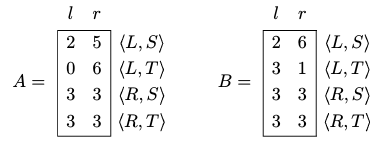
\includegraphics[width=.4\textwidth]{../img/strategic-form.png}
  \def\captionTitle{Left: An~extensive-form game. \\Right: The corresponding strategic-form pay-off matrices.}
  \caption[The strategic-form pay-off matrices]{\captionTitle{} \\(\cite[p.~67]{AGT07})}
  \label{fig:strategic-form}
\end{figure}

A~possible solution is to~use the \emph{sequence form} (\cite[pp.~70--73]{AGT07}).
This form of~\acrshort{lp} has variables just for \emph{sequences of~actions}.
Only sequences from~the same root-to-leaf paths are then combined:
\begin{figure}[H]
  \centering
  \tiny
  \def\svgwidth{.5\textwidth}
  \input{../img/strategic-form-tree.pdf_tex}
  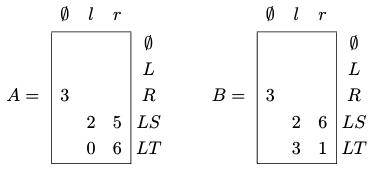
\includegraphics[width=.4\textwidth]{../img/sequence-form.png}
  \def\captionTitle{Left: A~game with sequences~$S_1 = \{\emptyset, L, R, LS, LT\}$ and $S_2 = \{\emptyset, l, r \}$.
    Right: The corresponding sequence-form pay-off matrices.}
  \caption[The sequence-form pay-off matrices]{\captionTitle{} (\cite[p.~67]{AGT07})}
  \label{fig:sequence-form}
\end{figure}
\noindent
\begin{itemize}
  \item \emph{Sequence}~$s_i(I)$ describes player~$i$'s history of~actions, i.e. edges passed along the path from the root to information set~$I\in I_i$.

    Set~$S_i$ denotes the set of~all $i$'s valid sequences:
    every non-empty sequence $s\in S_i$ is uniquely determined by its last action $a\in A_{I}$ at~an~information set~$I \in \I_i$.
    We can characterize
    \[
      S_i = \{\emptyset\} \cup \{ s_i(I) \cdot a \mid I\in\I_i,\, a\in A(I) \}
    \]
    which leads to the linear size $\lv S_i \rv = 1 + \sum_{I\in\I_i} \lv A(I) \rv$.

  \item The \emph{realization probability} (of~a~sequence~$s \in S_i$ under a~strategy~$\sigma_i \in \Sigma_i$) is $\pi^{\sigma_i} [s] = \prod_{a \in s} \pi^{\sigma_i}(a)$.

  \item Recall that a~mixed strategy~$\mu_1$ is a~probability distribution over (all) pure strategies of player~$1$.
    A~\emph{realization plan}\footnotemark{} $x\colon S_1 \to \R$ expresses the probability of~following sequence~$s$ under a~mixed strategy~$\mu_1$:
    \footnotetext{For player~$2$, a~realization plan $y\colon S_2 \to \R$ would be defined similarly.}
    \[
      x(s) = \sum _{\textrm{pure strategy } \sigma} \mu_1(\sigma)\; \pi^{\sigma}[s]
    \]
    If $\mu_1$ is a~behavior strategy and sequence~$s$ ends in a~state~$h$, we directly get $x(s) = \pi^{\mu_1}_1(h)$.
\end{itemize}

\section{Solving Games with Linear Programming}
{
  \setlength{\epigraphwidth}{0.65\textwidth}
  \epigraph{
    If you optimize everything, you will always be unhappy.
  }{Donald Ervin Knuth}
}%
Realization plans play the role of~variables in sequence-form \acrshort{lp} formulations.
We think of realization plans as vectors
$x := (x_s) _{s\in S_1} \in \mathbb{R} ^{\lv S_1 \rv}$
and
$y := (y_s) _{s\in S_2} \in \mathbb{R} ^{\lv S_2 \rv}$.
Not all vectors $x \ge 0$, $y \ge 0$ can be realization plans, though.
We need to add two more types of~\acrshort{lp} constraints.

The first kind of~necessary conditions states that the probability of~a~sequence can be decomposed into probabilities of~its immediate continuations:
\begin{align}
  \label{eq:seq-cond-children}
  \begin{split}
    x_{s_1(I)} &= \sum _{a \in A(I)}    x_{s_1(I \cdot a)}, \quad I\in\I_1, \\
    y_{s_2(I')} &= \sum _{a' \in A(I')} y_{s_2(I' \cdot a')}, \quad I'\in\I_2.
  \end{split}
\end{align}
The second kind of~conditions ensures that the probabilities in~realization plans sum to $1$:
\begin{equation}
  \label{eq:seq-cond-init}
  x_{\emptyset} = 1, \quad y_{\emptyset} = 1
\end{equation}
Interestingly, the conditions (\ref{eq:seq-cond-children}), (\ref{eq:seq-cond-init}) are also sufficient, giving a~full characterization for realization plans.~(\cite[Proposition~3.10, p.~71]{AGT07})

Now we re-formulate (\ref{eq:seq-cond-children}) and (\ref{eq:seq-cond-init}) using \emph{sequence constraint matrices}:
\begin{equation}
  \label{eq:seq-constraints}
  Ex = e, \ x \ge 0
  \quad \textrm{and} \quad
  Fy = f, \ y \ge 0.
\end{equation}
The first player gets a~sequence constraint matrix $E \in \{-1, 0, 1\} ^{(1 + \lv \I_1 \rv) \times \lv S_1 \rv}$, where columns are indexed by sequences from $s\in S_1$ and rows by equations of~(\ref{eq:seq-cond-children}) and (\ref{eq:seq-cond-init}).
Specifically, the first row of $Ex = e$ has form
\[
  x _{\emptyset} = 1,
\]
and the row corresponding to an~information set~$I \in \mathcal{I}_1$ looks like
\[
    x _{s_1 (I)} - \sum _{a \in A(I)} x _{s_1(I \cdot a)} = 0.
\]
The \emph{sequence constraint vector}~$e$ on the right-hand side is thus $(1, 0, \dots, 0) ^\top$.
Matrix~$E$ is sparse as it has only $\Onot(\lv \I_1 \rv + \sum_{I\in\I_i} \lv A(I) \rv)$ non-zero elements.
For constraints $Fy = f$, everything is analogous.

The \emph{sequence-form payoff matrix}~$A \in \mathbb{R} ^{\lv S_1 \rv \times \lv S_2 \rv}$ of~player~$1$ is described for every sequence $s \in S_1$ and $s' \in S_2$ by
\[
  A _{s,s'} = \sum _{\substack{z \in Z\\ s_1(z) = s,\; s_2(z) = s'}} \pi_c (z) \; u_1(z),
\]
where $\pi_c (z)$ is the contribution of~the chance to the probability, along the path to leaf~$z$.
The sequence-form payoff matrix of~player~$2$ is $-A$ from the zero-sum property.
Because the probability of~reaching any leaf~$z$ can be decomposed as
$
\pi^\sigma(z) =
\pi^{\sigma_1}[s_1(z)] \cdot
\pi^{\sigma_2}[s_2(z)] \cdot
\pi_c(z)
$,
we can write player~$1$'s utility as
\[
  u_1(\sigma)
  = \sum _{z \in Z}
  \pi^{\sigma_1}[s_1(z)] \cdot
  \pi^{\sigma_2}[s_2(z)] \cdot
  \pi_c(z) \cdot
  u_1(z)
  = \sum _{z \in Z}
  x_{s_1(z)}
  y_{s_2(z)}
  \pi_c(z) \,
  u_1(z)
  = x ^\top A y
\]
So a~best-response realization plan $x$ against arbitrary realization plan~$y$ maximizes the utility $u_1(\sigma) = x ^\top (Ay)$.
By~(\ref{eq:seq-constraints}), we can find such~$x$ as a~solution to this \acrshort{lp}:
\begin{equation*}
  \begin{split}
    \max\  &x^\top (Ay) \\
    E&x = e \\
    &x \ge 0.
  \end{split}
\end{equation*}
This is the corresponding dual \acrshort{lp} with a~vector of~dual variables $u \in \mathbb{R}^{1 + \lv \mathcal{I}_1 \rv}$:
\begin{equation*}
  \begin{split}
    \min\  &u^\top e \\
    E^\top &u \ge Ay.
  \end{split}
\end{equation*}

\clearpage
\todo

As both (\ref{seq-primal-param}) and (\ref{seq-dual-param}) are feasible, they have equal optimal values by the strong duality theorem.
Therefore, whereas player~$1$ wants to maximize $x^\top Ay = u^\top e$, his opponent wants to minimize it (in a~zero sum game) through his free choice of~$y$.
This amounts to the LP
\begin{equation}
\label{seq-dual}
\begin{split}
    \min_{u, y}\  &u^\top e \\
    E^\top u - Ay &\ge 0 \\
    Fy &= f \\
    y &\ge 0
\end{split}
\end{equation}
with the following dual LP
\begin{equation}
\label{seq-primal}
\begin{split}
    \max_{v, x}\  &v^\top f \\
    Ex &= e \\
    F^\top v - A^\top x &\le 0 \\
    x &\ge 0.
\end{split}
\end{equation}
It is important to mention that $E, F, A$ are sparse matrices, whose number of~variables and number of~non-zero values are linear in the size of~game tree.
In conclusion, zero-sum extensive form games can be solved using (dual) linear programming with LPs of~linear sizes.

\section{Solving Games with Learning Algorithms}
{
  \setlength{\epigraphwidth}{0.65\textwidth}
  \epigraph{
    Perfecting oneself is as~much unlearning as~it is learning.
  }{Edsger Wybe Dijkstra}
}%
\todo

\section{Subgames Revisited}

So far, the information sets have grouped only those states where the player was the acting player.
For the purposes of the subgame, it is also necessary to include the states that are indistinguishable from the point of view of other players.
Therefore, we define the \emph{augmented information sets} (\cite{BurchJohansonBowling13}):
\begin{defn}[augmented information set]
  For any player $i \in P$, let $H_i(h)$ be the sequence of player $i$'s information sets reached by player $i$ on the path to $h$, and the actions taken by player~$i$.

  Then \emph{augmented information set} $I_i(h)$ is defined by the following characterization:
  \[ I_i (h) = I_i (h') \; \Longleftrightarrow \; H_i (h) = H_i (h') \]
  for any two states $h, h' \in H$.
\end{defn}
At this point, we may finally define the notion of a~\emph{subgame} (\cite{BurchJohansonBowling13}):
\begin{defn}[subgame]
  \label{defn:subgame}
  An~(imperfect-information) \textbf{subgame} is a~forest of~subtrees, closed under both the descendant relation and membership within augmented information sets for any player.
\end{defn}
Consult Section~\ref{sec:naive-rps-subgame} for an~illustrative example.

\subsection{Previous Works}
